\section{Mise en œuvre}

\subsection{Grapher}
Il était important dès le début du projet de visualiser de manière claire les 
informations liées aux translation et rotations des articulations les unes par 
rapport aux autres. Unity s'avère être une contrainte pour ceci~: il est difficile
de faire une rendu de primitives géométriques (lignes, triangles) directement. Il
a donc fallu passer en contorsionniste à travers un ensemble d'objets LineRenderer.

\begin{figure}[h!]
\centering
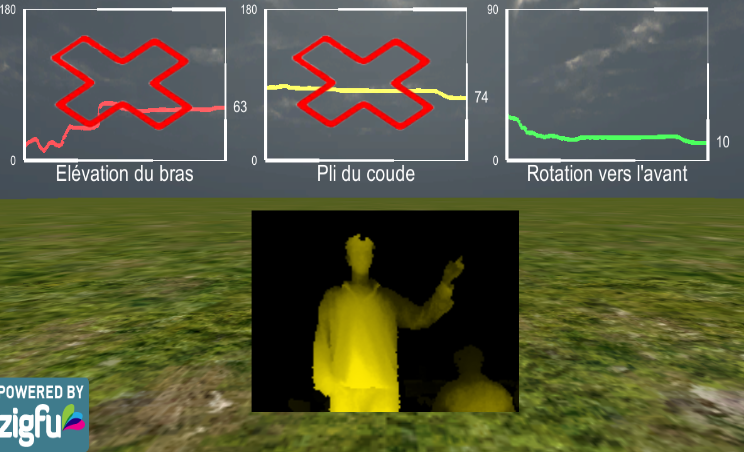
\includegraphics[width=\linewidth]{../images/zfm_graph}
\caption{Graphs de Zigful-Meyer.}
\end{figure}

Le résultat est une classe permettant de faire de manière simple et flexible des
graphes au sein de Unity. Initialement qu'un outil pour faciliter le 
débuggage, nous avons finalement décidé de les garder dans le projet afin de
fournir un retour d'information riche et continue au patient. Sont donc présentées 
à l'écran à la fois la progression (par exemple, l'élévation du bras) et les 
contraintes à ne pas briser.
    
\subsection{Multi Camera}
Afin d'augmenter la lisibilité des graphes, nous avons réfléchi à un moyen de les afficher de manière séparée du reste de
l'environnement 3D. Notre première idée était tout simplement de créer ces graphiques dans une GUI 2D, en premier
plan de l'application. Malheureusement, il n'est pas possible avec Unity de dessiner des courbes en 2D, et les différentes
options du GUILayer ou UnitGUI ne nous permettaient pas d'arriver à un résultat équivalent.\\
Il est en revanche possible de multiplier les caméras, et de choisir si celle-ci doivent utiliser ou non la projection 3D. Nous 
avons vu là la possibilité de "construire" notre GUI de toute pièce, et de le projeter simultanément avec la scène grâce à
l'utilisation d'une caméra supplémentaire. La "ruse" est alors de créer la  \textit{GUIscène} dans un endroit inutilisée de la 
scène, de centrer en face une caméra immobile, et de dessiner en 3D les courbes que nous désirons.
\begin{figure}
\begin{center}
  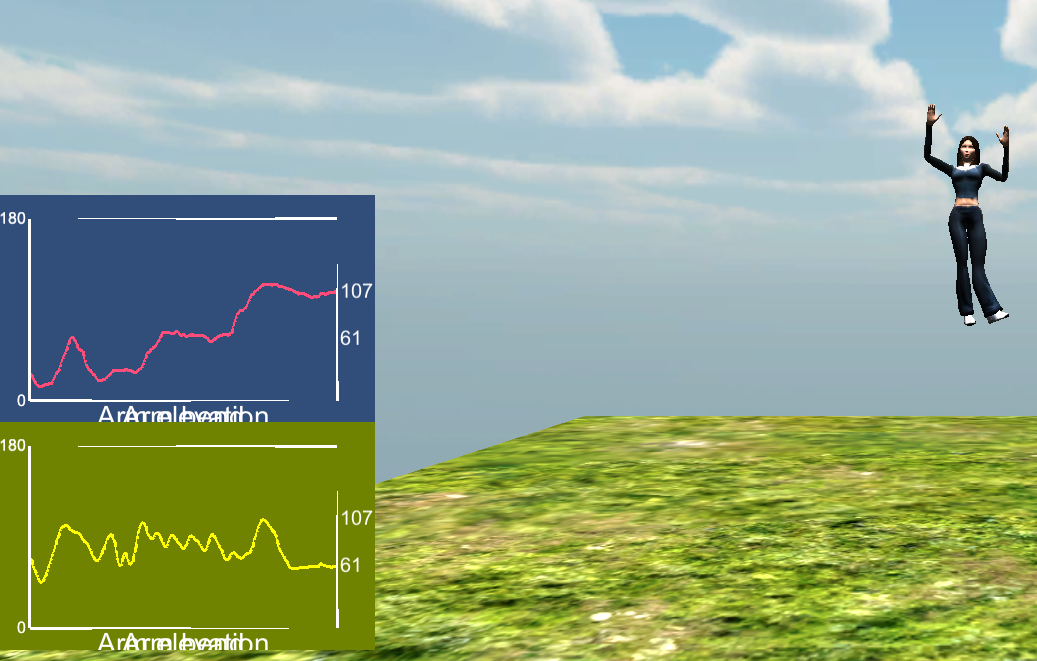
\includegraphics[scale=0.6]{../images/multicamera.png} \caption{Multi camera pour affichage des graphes}
  \end{center}
\end{figure}
 On notera un petit problème d'affichage des légendes, dû à l'utilisation de GUIText, texte ayant la particularité d'être partagé par toutes les 
caméras disposant d'un GUILayer. Il suffirait de rendre aussi ces textes en 3D pour palier au problème.

\subsection{Avatar 3D}   
Un point important de tout jeu, est l'aspect de ou des avatars qu'est amené à contrôler le joueur. C'est en effet à lui que va devoir s'identifier le joueur. Dans notre, l'avatar est d'autant plus important qu'il se veut être le double virtuel du joueur / patient. Il était donc important pour nous d'arriver à proposer un modèle 3D pour le personnage, et d'arriver à faire correspondre ses mouvements avec ceux du joueur par l'intermédiaire du Kinect. Ici nous avons récupéré le mesh 3D et les textures du personnages fournis dans les samples de Zigfu. Il faut ensuite faire le \textit{rigging} entre les bones du squelette et le mesh3D. La dernière étape a consisté à lier notre script de contrôle au personnage.
\begin{figure}
\begin{center}
  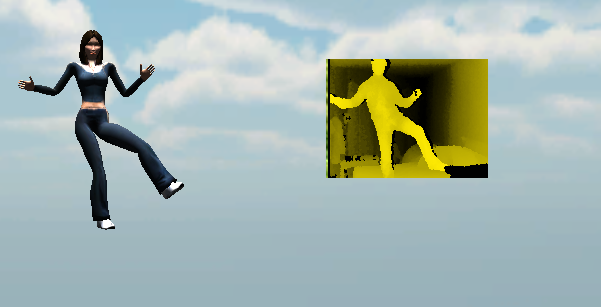
\includegraphics[scale=1]{../images/avatar3D.png} \caption{Relation entre le joueur et son \textit{double} numérique}
\end{center}
\end{figure}

    
\subsection{Menu}

Pour le menu nous avons décidé de ne pas utiliser le contrôle par la Kinect.
D'abord si le patient a besoin de faire le test il n'a peut être pas la
mobilité nécessaire pour faire les manipulations, qui tendent à être assez 
facile à échouer. Nous avons eu une difficulté non-triviale à utiliser les menus
proposés dans les samples de Zigfu alors que n'avons pas de problèmes moteurs.
Il ne faudrait surtout pas que le patient soit frustré avant même le début de
l'exercice.
    
\begin{figure}[h!]
\centering
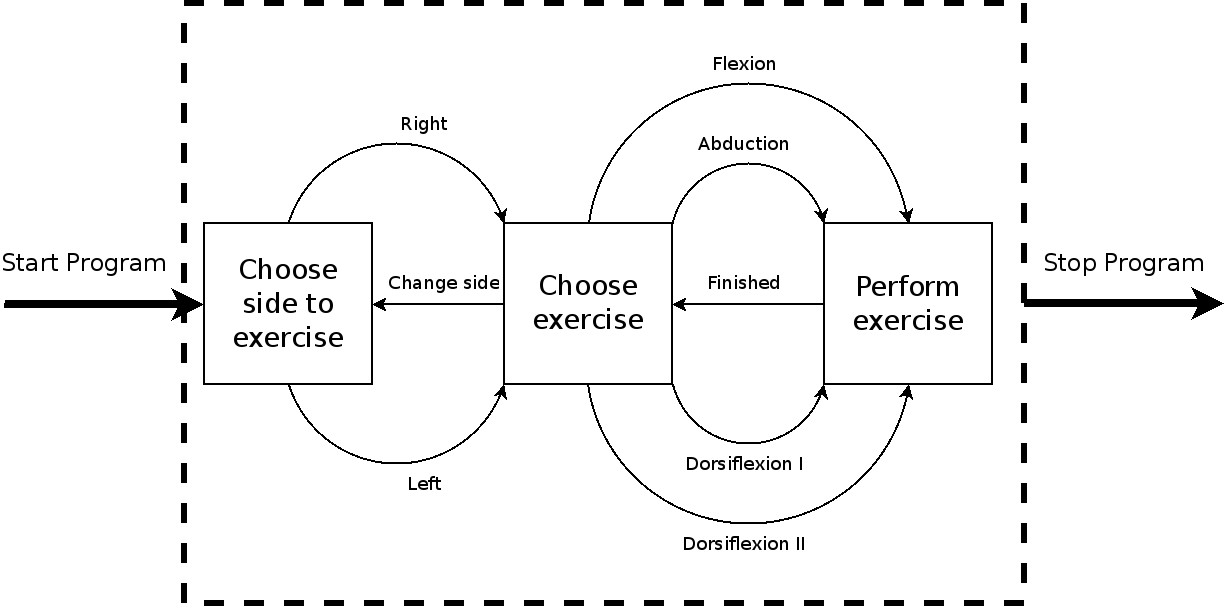
\includegraphics[width=\linewidth]{../images/menu}
\caption{Machine à états de la Menu.}
\end{figure}

Le cas d'utilisation imaginé comporte en plus un médecin, qui sera justement là
pour lancer les exercices et donner des conseils précis alors que le système 
se contente de mesurer la progression de manière précis.

\begin{figure}[h!]
\centering
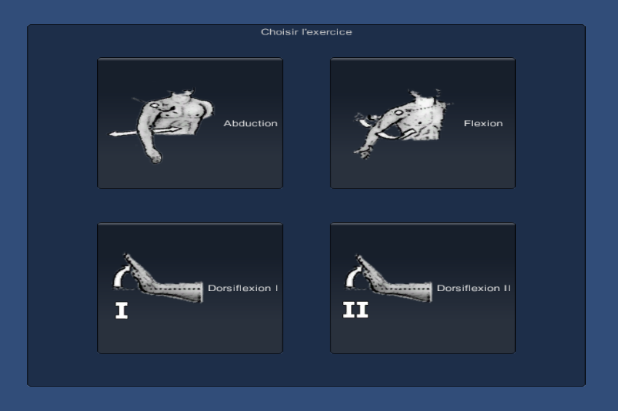
\includegraphics[width=0.8\linewidth]{../images/menu2}
\caption{Capture d'écran d'un des pages du menu.}
\end{figure}
    

\subsection{ExerciseMonitor}

Tous les exercices présentés suivent un schéma commun~: le patient commence dans
une position donnée et doit faire, au mieux qu'il peut, un mouvement. Ce mouvement
est souvent contraint par un nombre de critères~: il ne doit pas, par exemple,
plier son coude en levant son bras. Nous avons pu noter que les spécialistes 
mettent directement un 0
(disqualification) pour l'exercice si la contrainte est brisée!

\begin{figure}[h!]
\centering
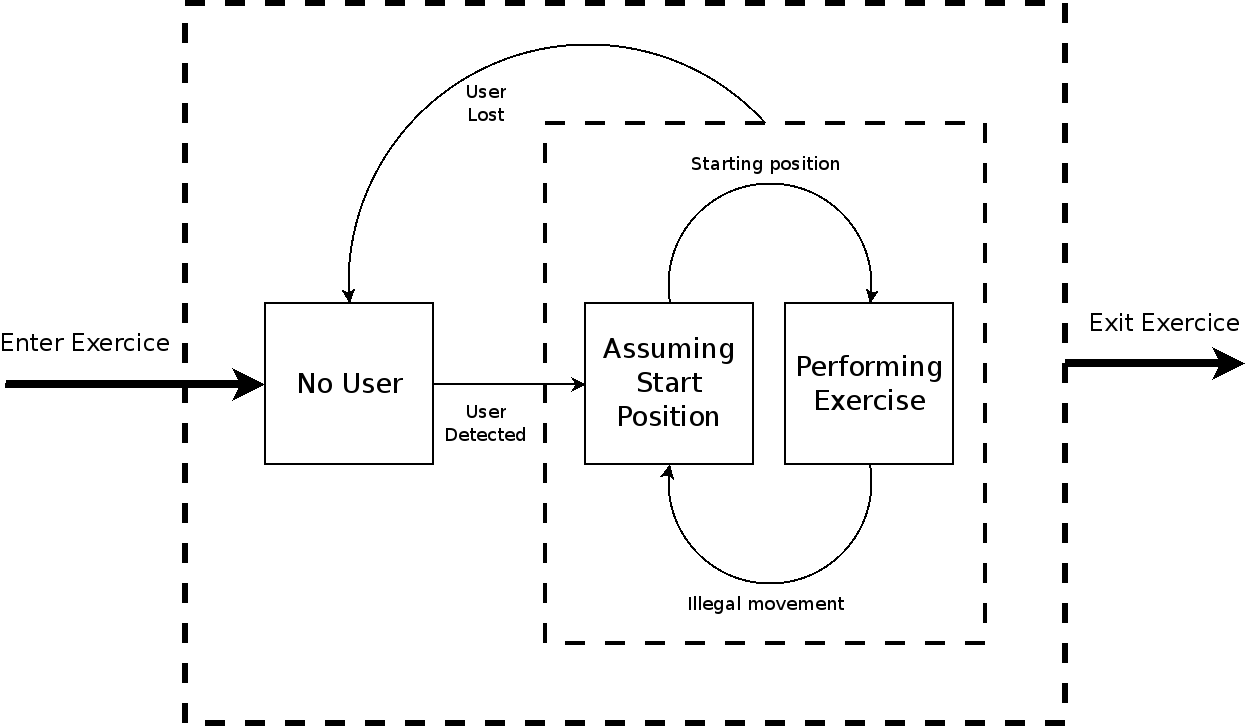
\includegraphics[width=0.9\linewidth]{../images/exercise_monitor}
\caption{Machine à états de la ExerciseMonitor.}
\label{fig:exercise_monitor}
\end{figure}

Notre système n'éjectera pas le patient de l'exercice avec un 0 dès qu'il brise 
une contrainte, mais sa progression sera bloquée. Il aura besoin de revenir à la
position initiale pour recommencer l'exercice, mais pourra le refaire autant de fois
qu'il veut. Pour gérer cette boucle d'échec et de relance, une machine à états
hiérarchique est utilisée (voir la figure \ref{fig:exercise_monitor}.
    